\section{An audited margin vector with a neural proposal model}\label{sec:neural}

A release decision needs a measured quantity, not a score. For a proposed mechanism
$\theta$, let $j=(a,h,g,v)$ index an adversary, harm class, target group and
release vintage, including a separate index for an attacker pooling vintages.
The finite, declared index set is $\mathcal J$, of cardinality $n$. A scenario
$j$ fixes the target sampling frame, attack algorithm, access to auxiliary
information, release programme and binary definition of success. Conditional
on a fixed proposed release and these specifications, let $P_{\theta j}$ be
the law of one fresh attack experiment and define the actual risk
$r_j(\theta)=\E_{P_{\theta j}}S_j$, where $S_j\in\{0,1\}$ records success.
The tolerance $\tau_j\in(0,1)$ is fixed before the final audit. A population
average and a particular target require distinct scenario definitions.
A neural score does not supply this quantity. We call the vector of
independently audited margins the \emph{audited margin vector}, and its
smallest entry the \emph{minimum audited margin}:
\begin{equation}
 {\bf z}(\theta)=\left(1-\frac{\overline r_j(\theta)}{\tau_j}
                  \right)_{j\in\mathcal J}\in\mathbb R^n,
 \qquad T(\theta)=\min_{j\in\mathcal J}z_j(\theta).
 \label{eq:trust-position}
\end{equation}
Here $\overline r_j$ is a simultaneous upper confidence bound, with its sampling
unit and adversary written into the assessment. A nonnegative $T$ means every
declared coordinate passes. The complete vector must accompany the scalar: the
minimum alone conceals which group or programme attack constrains the release.
Utility $U(\theta)$ is kept as a separate coordinate, since a release can have
large audited margins while carrying little public value. Missing or
unaudited coordinates receive $\overline r_j=1$ and therefore fail whenever
$\tau_j<1$. Each assessment thus starts with no inherited claim of safety:
collect independent evidence, tighten the bounds, improve the mechanism, and
recertify. It does not promise that evidence will rescue an unsafe release.

Figure \ref{fig:trust-vector} depicts the coordinatewise decision. Each entry
is a separately audited margin, and one negative entry forces the minimum
below zero even if the other coordinates pass.
\begin{figure}[H]
\centering
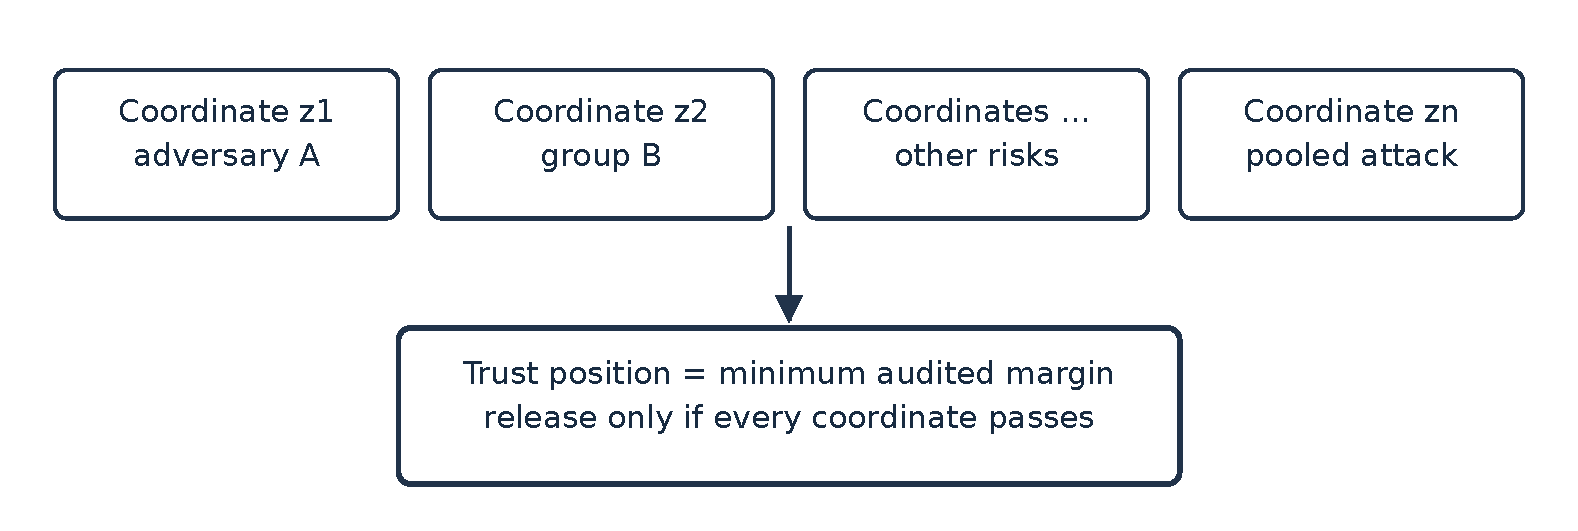
\includegraphics[width=.94\linewidth]{diagrams/trust_vector.pdf}
\caption{The $n$-dimensional trust position uses independently bounded risk coordinates $z_j=1-\overline r_j/\tau_j$. The labels illustrate declared coordinates, not numerical results.}
\label{fig:trust-vector}
\end{figure}


\subsection{The neural model and what its output means}

Encode a proposed release and its environment as $x(\theta)\in\mathbb R^d$:
mechanism parameters, sample fraction, key entropy and sparsity, auxiliary
information quality, number and overlap of prior releases, access controls,
population shifts and target-group indicators. All features must be available
\emph{before} certification and their provenance recorded. A transparent
baseline is a regularised logistic model; our nonlinear proposal model is
\begin{align}
 H_0&=x, &H_{\ell+1}&=\rho(H_\ell W_\ell+b_\ell),\quad 0\leq\ell<L,\\
 \widehat{\boldsymbol r}_{\phi}(x)
   &=\sigma(H_LW_{\rm out}+b_{\rm out})\in(0,1)^n,
 &\mathcal L(\phi)&=-\sum_{i,j}w_{ij}
  [y_{ij}\log\widehat r_{ij}+(1-y_{ij})\log(1-\widehat r_{ij})].
 \label{eq:neural-risk}
\end{align}
The \texttt{neural\_trust} module fixes $L=1$; \texttt{sentry\_r} makes $L$
configurable.
The label $y_{ij}$ is the \emph{observed success of an attack} on a separate
scenario draw, with a zero label for a failed or abstaining attack as specified
in the threat model. Unevaluated pairs have $w_{ij}=0$; repeated attacks sharing
one auxiliary file are clustered by file rather than treated as independent.
The sigmoid outputs are predicted attack frequencies, not audited margins or
probabilities that a release is safe, and no ordering of them across harm classes is implied.
Train on past mechanism--adversary scenarios, hold out whole populations,
release programmes and vintages, and keep the final audit draws out of all
training, tuning, calibration and feature selection. Compare log loss, Brier
score and reliability diagrams with the logistic and frequency baselines, both
overall and by group \citep{guo2017}. A calibration plot is a diagnostic, never a certificate
for the highest-risk individual.

The neural model proposes a \emph{finite} shortlist $\Theta_0$: it ranks
candidates by their largest predicted risk-to-tolerance ratio; utility enters
only the final choice among certified candidates. For each candidate and $j$, run $B_{\theta
j}$ fresh, conditionally identically distributed Bernoulli attacks and count
$K_{\theta j}$ successes. Fix the sample sizes before observing final outcomes.
With $M=|\Theta_0|n$ prespecified inspected coordinates,
define the exact one-sided bound
\begin{equation}
 \overline r_{\theta j}=
 \begin{cases}
 1,&K_{\theta j}=B_{\theta j},\\
 F^{-1}_{\mathrm{Beta}(K_{\theta j}+1,\,B_{\theta j}-K_{\theta j})}
      (1-\alpha/M),&K_{\theta j}<B_{\theta j}.
 \end{cases}\label{eq:neural-audit}
\end{equation}
Certification uses \eqref{eq:trust-position} and \eqref{eq:neural-audit}, never
the neural output. The final choice may maximise $U$ among certified candidates,
provided the shortlist was fixed without looking at these final audit draws.

Figure \ref{fig:neural-workflow} makes the separation between development
and final evidence explicit. The arrows into the final gate carry audit
bounds and tolerances; the network contributes only the fixed shortlist.
\begin{figure}[H]
\centering
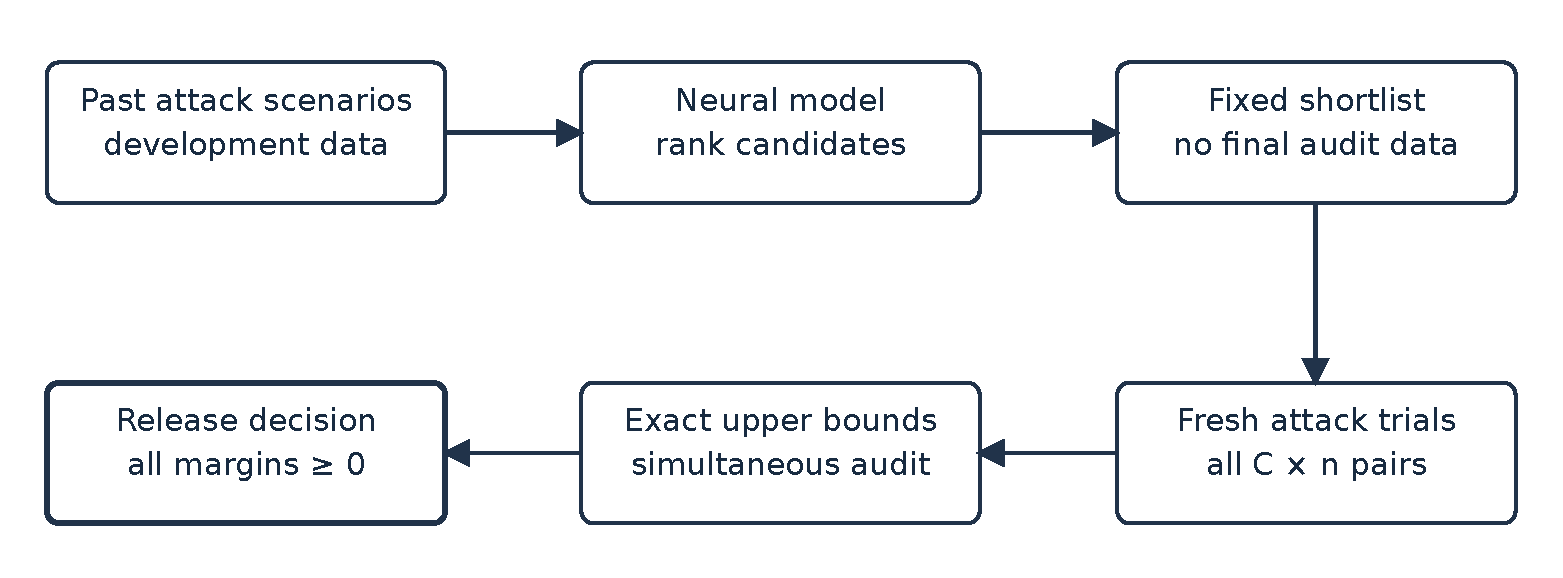
\includegraphics[width=.94\linewidth]{diagrams/neural_workflow.pdf}
\caption{The neural network ranks candidates; independent attack trials and exact simultaneous upper bounds decide. $C=|\Theta_0|$ and $n$ is the number of risk coordinates.}
\label{fig:neural-workflow}
\end{figure}


\begin{proposition}[Selection-safe finite-family certification]\label{prop:neural-gate}
Condition on development information $\mathcal D$ and its resulting finite
shortlist, candidate releases, scenarios and sample sizes. Suppose each final
audit count is $\mathrm{Binom}(B_{\theta j},r_j(\theta))$ conditional on
$\mathcal D$; auxiliary information sampled afresh is included in this
experiment, whereas fixed auxiliary information is conditioned upon. Then
with probability at
least $1-\alpha$, simultaneously for every inspected pair,
$r_j(\theta)\leq\overline r_{\theta j}$. Consequently the rule selecting any
candidate with $T(\theta)\geq0$ has probability at most $\alpha$ of certifying
a candidate whose risk exceeds a declared tolerance in any coordinate.
\end{proposition}
\begin{proof}
For one pair the event that the exact upper bound falls below the true risk
has probability at most $\alpha/M$ by inversion of the binomial lower-tail
test (Appendix \ref{app:neural}). A union bound over the $M$ pairs gives the
simultaneous statement, without requiring independence between pairs. On this
event every certified candidate satisfies $r_j(\theta)\leq\tau_j$ for all
$j$, regardless of which certified candidate the final rule selects.
Taking expectation over $\mathcal D$ gives the unconditional guarantee.
\end{proof}

If the release, attack, shortlist or group definitions change in response to
final outcomes, the conditional argument no longer applies. Freeze and restart
with untouched audit draws, or replace the fixed-sample bound by the anytime
procedure of the main text (the section on adaptive attacks and anytime-valid certification) with an explicit multiplicity
allocation. Binomial sampling covers attack-draw variability conditional on a
fixed population and mechanism. It does not cover uncertain input data, unknown
auxiliary sources, a stronger future attacker or distribution shift. Those are
separate scenario coordinates or require a stated outer uncertainty analysis.

\subsection{What changes as the dimension grows}

The number $d$ of input features and the number $n$ of risk coordinates are
different. For widths $q_0=d,q_1,\ldots,q_L,q_{L+1}=n$, a dense forward pass
costs $O(\sum_{\ell=0}^{L}q_\ell q_{\ell+1})$ operations per scenario and
stores $O(\sum q_\ell q_{\ell+1})$ parameters; a training epoch multiplies
the cost by the number of labelled scenarios. Sparse embeddings or shared
encoders can reduce cost when many groups share structure, but cannot supply
evidence in an unseen group. A full final audit over $C$ candidates and $n$
coordinates uses $Cn$ confidence bounds and, at zero observed successes in
every coordinate, needs at least
\begin{equation}
 B\geq\left\lceil\frac{\log(\alpha/(Cn))}{\log(1-\tau_{
 \min})}\right\rceil\label{eq:neural-budget}
\end{equation}
independent trials per coordinate to certify a common minimum tolerance
$\tau_{\min}$. This is necessary and sufficient when that coordinate has
zero successes; with successes, more trials can be needed. Thus computational
amortisation by a network
does not erase the statistical cost of many simultaneous guarantees.
For an $L$-Lipschitz risk function on $[0,1]^d$, even a direct grid at
accuracy $\epsilon$ uses order $(L/\epsilon)^d$ cells. Without such
regularity, finite observations alone cannot guarantee uniform pointwise
accuracy. Report learning curves against both $d$
and $n$; do not describe merely adding hidden units as solving this problem.

For stress testing, if the full law $Q_{\theta j}$ of the deployed attack
experiment is known to satisfy
$\mathrm{TV}(P_{\theta j},Q_{\theta j})\leq\delta_j$,
bounded attack success gives
$r_{Q_{\theta j}}(\theta)\leq r_{P_{\theta j}}(\theta)+\delta_j$.
A declared and justified
bound can therefore replace $\overline r_j$ by
$\min(1,\overline r_j+\delta_j)$. Estimating $\delta_j$ from a neural
embedding alone does not justify that guarantee. Out-of-scope feature values,
new linkage data and an unbounded shift require refusal and a new assessment.

The testable methodological contribution is the combination of an audited
margin vector, a neural search model, and an independent simultaneous audit
under adaptive choice of the final candidate. Neural prediction, binomial
bounds and neural calibration individually have extensive precedents
\citep{bates2021,guo2017}; the
claim here is about their stated division of labour for a release programme,
not an untested claim of superior empirical performance. The accompanying
\texttt{privacy\_risk.neural\_trust} module includes a seeded synthetic demonstration of the search
and audit interface. It cannot validate the existing tables in this paper.
An empirical extension must preregister targets and populations, compare the
network with the logistic and frequency baselines at fixed audit budgets,
report selective utility and worst-group failures, and rerun every pooled
attack on held-out real programmes.
